
\section*{Problem 1}

\noindent
\textbf{Data Collection}

The data are all downloaded from CSMAR as required by the problem, namely the closing index over 2003/12/31 to 2023/12/31 (the data is 2003 is for calculating the return in 2004/01). 

\\

\noindent
\begin{Question} 


\noindent
\textbf{Claim} 

The downloaded data are daily returns, but the question asks to derive monthly returns. Here, I use the daily returns in the last day of each month to represent the monthly returns. As this is not specifically identified in the question, I believe all methods including taking average and last-day-return work.


\noindent
\textbf{Steps} 

\textit{Data Manipulation.} I convert the `date' column from object to datetime format and then changing it to a monthly period, as it works better for time-series data.


\textit{Return Calculation.} First the data with index code ``000300" (standing for CSI 300) is taken out for calculation. The monthly return is derived by $.pct\_change()$ method (whose algorithm is exactly the same as the provided formula). Then the 2005-04 data is dropped as this is the first index data, with no return.


\noindent
\textbf{Results} 

\textit{Summary Statistics.} By using library $scipy.stats$, we can get the data required.

\begin{table}[htbp]
    \centering
    \caption{Summary Statistics}
    \vspace{0.4cm}
    \csvautotabular{data/index_stats.csv}
\end{table}

\end{Question}



\noindent
\begin{Question} 

The graph is shown in the next page.
\end{Question}



\noindent
\begin{Question} 

By analyzing the figure data from (b), the skewness value is relatively large but near zero, suggesting that the data distribution is nearly symmetrical, which is in accordance with normal distribution. The kurtosis value is notably lower than that of a normal distribution, suggesting that the data exhibits a heavy-tailed distribution.

Being more rigorous, based on the Shapiro-Wilk test, the p-value is less than the typical significance level of 0.05. This indicates strong evidence against the null hypothesis that the data follows a normal distribution. Therefore, returns of the CSI300 index is NOT normally distributed.


\begin{table}[htbp]
    \centering
    \caption{Shapiro-Wilk Test Statistics}
    \vspace{0.4cm}
    \csvautotabular{data/test_stats.csv}
\end{table}


\noindent
\textit{Graph.} Histogram as shown below, from 2005 -- 2023.

\begin{figure}[h]
\centering
\vspace{-0.43cm}
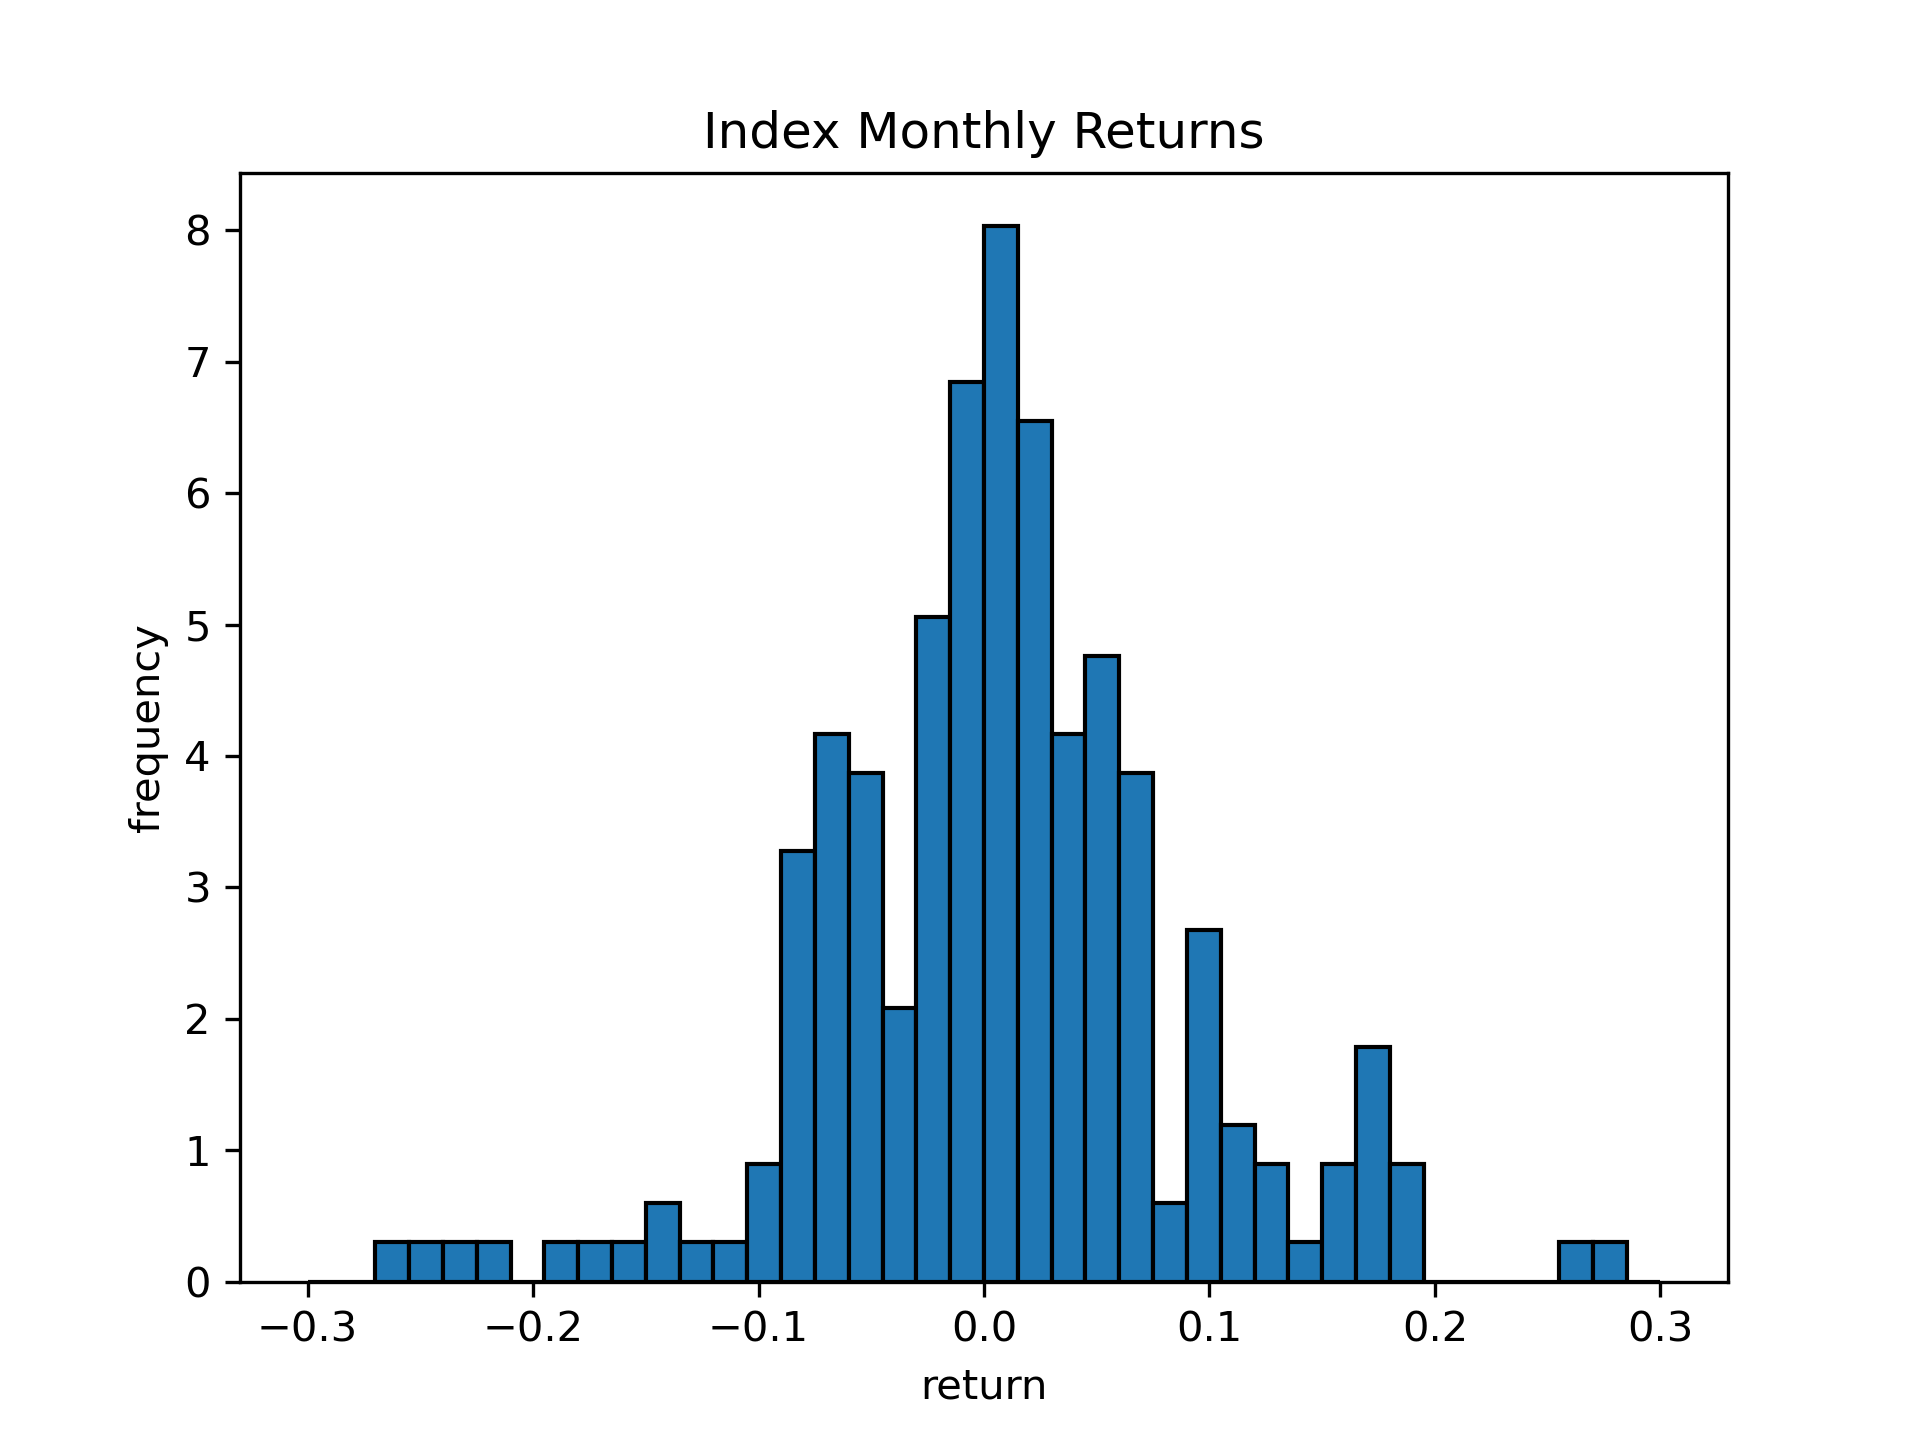
\includegraphics[width=0.85\textwidth]{data/q1_graph.png}
\caption{Histogram for CSI 300 monthly returns}
\label{fig:example}
\end{figure}

\end{Question}